\documentclass[sigconf,review]{acmart}

\settopmatter{printacmref=true}
\setcopyright{none}
\renewcommand\footnotetextcopyrightpermission[1]{}
\pagestyle{plain}

\title{FounderBench: Evaluating LLM Agents on Sequential Startup Decisions}

\author{Yufeng Wang}
\affiliation{%
  \institution{Independent Researcher}
  \country{United States}}
\email{louiswang524@gmail.com}
\renewcommand{\shortauthors}{Yufeng Wang}

\begin{abstract}
Existing agent benchmarks emphasize tool use, web navigation, and software editing, but rarely isolate repeated operating decisions under scarce resources and delayed consequences.
We introduce FounderBench, a controlled benchmark for startup-like sequential decision making.
Given a simulated company state and noisy market information, an agent must choose from 13 structured business actions over a fixed horizon; a deterministic simulator updates cash, demand, quality, and risk, and task-specific code maps final outcomes to a 0--100 score.
Free-form rationale is logged for audit but never scored.
The suite contains 50 synthetic public tasks balanced across 10 operating families.
\textbf{Headline gap:} a task-aware calibration policy averages 80.90 (37/50 solved), while the best hosted single run reaches only 67.69 (32/50); no human-founder baseline is reported.
Rankings reverse between average score and solved count, and family profiles expose distinct operating failures.
We release tasks, simulator and scoring code, adapters, validated task-level results, and generation scripts.
All hosted rows are single runs on visible public tasks; scores do not establish real-world startup competence.
\end{abstract}

\keywords{LLM agents, benchmark, sequential decision making, simulation, business operations, outcome-based evaluation}

\begin{CCSXML}
<ccs2012>
 <concept>
  <concept_id>10010147.10010257.10010293.10011809</concept_id>
  <concept_desc>Computing methodologies~Planning under uncertainty</concept_desc>
  \concept_significance>500</concept_significance>
 </concept>
 <concept>
  <concept_id>10010147.10010257.10010321</concept_id>
  <concept_desc>Computing methodologies~Intelligent agents</concept_desc>
  \concept_significance>300</concept_significance>
 </concept>
</ccs2012>
\end{CCSXML}
\ccsdesc[500]{Computing methodologies~Planning under uncertainty}
\ccsdesc[300]{Computing methodologies~Intelligent agents}

\begin{document}
\maketitle

\section{Introduction}
Agent evaluation has moved from short answers toward interactive settings where a model must observe state, choose actions, and accept consequences~\cite{liu2025agentbench,mialon2023gaia,jimenez2024swebench,zhou2024webarena,yao2024taubench,merrill2026terminalbench,li2026lhtb}.
Recent long-horizon suites further stress sustained CLI execution~\cite{merrill2026terminalbench,li2026lhtb}, policy-rich enterprise workflows~\cite{chen2026chibench}, multi-agent economies~\cite{sugiura2026coffeebench}, and long-game startup/CEO coherence~\cite{he2026ycbench,chen2026ceobench}.
These benchmarks are valuable, yet a complementary operating regime remains underexplored: short, family-labeled startup decisions under scarce resources and delayed consequences, scored by inspectable outcome functions rather than open-ended tool traces or year-end cash alone.

That gap matters because persuasive text is easy to confuse with competence.
Consider a Demo Day episode: an agent may write a confident fundraising narrative while never researching markets, under-improving offer quality, and exhausting cash on poorly timed campaigns; the simulator records a weak state and the family scorer returns a low outcome even though the prose looked founder-ready.
Startup-like decisions couple research, acquisition, retention, pricing, pivots, and fundraising under a single budget.
Evaluating them requires an environment where actions change state and outcomes---not rhetoric---determine score.

FounderBench is designed for that setting (Figure~\ref{fig:loop}).
Each episode provides a structured company observation and a fixed action vocabulary.
The agent returns a JSON action list; a deterministic simulator applies costs and transitions; task-specific scoring code returns a 0--100 outcome score.
The design follows a simple principle used by strong execution benchmarks: make success checkable without grading free-form prose~\cite{jimenez2024swebench,zhou2024webarena,mialon2023gaia}.

Relative to prior agent suites, FounderBench deliberately trades open-world breadth for inspectable operating tradeoffs.
Tasks are synthetic and fully public; transitions and scores can be replayed; calibration policies establish a capability ladder before hosted models are interpreted.
Empirically, the ladder is wide: task-aware calibration reaches 80.90 average score (37/50 solved), while the best hosted single run reaches 67.69 (32/50), with the largest hosted deficits on pivot and Demo Day families.
The resulting test asks whether an agent can turn noisy observations into sequenced business actions under binding constraints.

Our contributions are:
\begin{itemize}
  \item \textbf{Benchmark.} A 50-task suite spanning 10 startup operating families, with fixed seeds, 13 structured actions, and visible task definitions.
  \item \textbf{Outcome protocol.} A deterministic simulator and task-specific scorers that evaluate final state rather than rationales, keeping provider outputs comparable.
  \item \textbf{Empirical baselines.} Validated single-run results for eleven hosted configurations and four calibration policies, with family diagnostics and provider-error reporting.
  \item \textbf{Auditable release.} Task-level evidence, adapters, validation, task-mix analyses, datasheet-style documentation, and generators that regenerate every reported table and figure.
\end{itemize}

FounderBench is a controlled synthetic test of sequential decisions.
It is not evidence that a model can run a real company: there is no human-founder calibration and no official hidden leaderboard, and the present hosted numbers are single runs on visible public tasks.

\section{Related Work}
\paragraph{Interactive, terminal, and sequential agents.}
ReAct~\cite{yao2023react} and Toolformer~\cite{schick2023toolformer} established reasoning--action loops; Voyager~\cite{wang2023voyager} studied open-ended long-horizon play.
AgentBench~\cite{liu2025agentbench} and GAIA~\cite{mialon2023gaia} broaden interactive evaluation, while SWE-bench~\cite{jimenez2024swebench}, WebArena~\cite{zhou2024webarena}, and $\tau$-bench~\cite{yao2024taubench} emphasize executable correctness.
Terminal-Bench~\cite{merrill2026terminalbench} and Long-Horizon Terminal-Bench~\cite{li2026lhtb} push this further into containerized CLI work lasting tens to hundreds of steps.
Agentick~\cite{creus2026agentick} unifies sequential decision-making evaluation across RL, LLM, and hybrid agents with delayed rewards and oracle-normalized scores.
FounderBench shares the executable-outcome principle but specializes to startup operating decisions with a fixed structured action schema rather than shell, code, browser, or cross-paradigm Gym tasks.

\paragraph{Workplace, enterprise, and startup simulations.}
TheAgentCompany~\cite{xu2025theagentcompany} and WorkArena~\cite{drouin2024workarena} evaluate workplace and enterprise web tasks; EconWebArena~\cite{liu2026econwebarena} and EnterpriseArena~\cite{han2026enterprisearena} study economic and CFO-like allocation; $\chi$-Bench~\cite{chen2026chibench} stresses policy-dense healthcare workflows.
CoffeeBench~\cite{sugiura2026coffeebench} is a complementary economic sandbox: a heterogeneous multi-agent coffee supply chain where agents maximize net income via negotiation, cash, and inventory over 90 days.
AgentHire-Bench~\cite{agenthire2026} evaluates managerial intelligence across hiring, delegation, management, and review---a richer view of team building than FounderBench's coarse \texttt{hire\_agent} action.
BrandEval~\cite{brandeval2026} stress-tests risk-sensitive crisis communication under trust and reputation dynamics, motivating future FounderBench scenarios with sharper reputation-risk shocks.
Closest agentic startup operators are YC-Bench~\cite{he2026ycbench} (one-year CLI startup, final funds) and CEO-Bench~\cite{chen2026ceobench} (500-day CEO simulation with pricing, marketing, budgeting, and programmable tools, scored by ending cash).
Separately, Benhenda's YC Bench~\cite{benhenda2026ycbenchforecast} is \emph{predictive} rather than agentic: it forecasts Y Combinator batch outperformance from public signals, reminding us that ``outcome-based'' can mean forecasting real startups as well as scoring simulated decisions.
FounderBench is complementary along three axes (Table~\ref{tab:related}): short, family-labeled episodes ($\leq$10 weeks) instead of one continuous long game; a fixed structured action schema instead of open CLI/code tools; and task-specific 0--100 scorers plus calibration policies instead of year-end cash or net income alone.
The goal is family-level diagnosis of operating failures under a shared, inspectable interface.

\begin{table*}[t]
\caption{Positioning against nearby agent and business benchmarks. Oracle: what is graded. Human?: reported human/expert baseline. Hidden?: private/held-out tasks used for official hosted scores in the paper.}
\label{tab:related}
\centering\scriptsize
\begin{tabular}{p{1.7cm}p{1.55cm}p{1.35cm}p{1.55cm}p{1.55cm}cc}
\toprule
Benchmark & Domain & Horizon & Interface & Oracle & Human? & Hidden? \\
\midrule
YC-Bench~\cite{he2026ycbench} & startup ops & $\sim$1 year & CLI & final funds & no & no$^\dagger$ \\
CEO-Bench & startup CEO & 500 days & tools/code & ending cash & no & no$^\dagger$ \\
CoffeeBench & multi-agent economy & 90 days & tools & net income & no & no$^\dagger$ \\
WebArena~\cite{zhou2024webarena} & web tasks & multi-step & browser & functional checks & yes & partial \\
SWE-bench~\cite{jimenez2024swebench} & GitHub issues & patch & code & unit tests & no & no \\
FounderBench & startup families & $\leq$10 weeks/ep. & structured JSON & family $0$--$100$ state & no & frozen$^\ddagger$ \\
\bottomrule
\end{tabular}
\begin{flushleft}\vspace{-0.4em}\scriptsize
$^\dagger$As reported in the cited papers' primary public evaluations.
$^\ddagger$Private holdout is frozen with fingerprints; this paper reports hosted scores only on the visible public suite.
\end{flushleft}
\end{table*}

\paragraph{Documentation and evaluation practice.}
Datasheets~\cite{gebru2021datasheets} and HELM~\cite{liang2023holistic} motivate transparent documentation and multi-metric reporting.
We follow that practice with a datasheet, raw task-level outputs, and diagnostics that separate strategic weakness from interface failure without inventing corrected counterfactual scores.

\paragraph{Executable judging versus LLM judges.}
Outcome-only scoring is a deliberate alternative to rubric or LLM-as-a-judge pipelines.
RULERS~\cite{hong2026rulers} shows that even structured rubrics need locked criteria and evidence anchoring to resist scoring drift; FounderBench sidesteps that class of fragility by never grading free-form text.
Complementary work shows LLM judges can be manipulated by short adversarial strings~\cite{zhao2025onetoken}, reinforcing why persuasive rationales are logged for audit but excluded from $f_i$.
Hybrid designs---proxy state checks, partial human review, or stochastic market noise---can trade determinism for realism; we discuss that design space in Section~\ref{sec:design-properties} and leave seeded ecological variants to future work.

\section{Benchmark Design}
\subsection{Benchmark desiderata}
\label{sec:desiderata}
Before detailing mechanics, we state five desiderata that guided FounderBench (inspired by desiderata-first agent benchmarks~\cite{xu2025theagentcompany,zhou2024webarena}):
\begin{enumerate}
  \item \textbf{Executable outcomes.} Success must be checkable from simulator state, not prose quality~\cite{jimenez2024swebench,zhou2024webarena,mialon2023gaia}.
  \item \textbf{Family diagnosis.} The suite should expose \emph{which} operating failure modes matter, not only a single scalar.
  \item \textbf{Shared interface.} Providers must face identical observations and action schemas so differences are attributable to policy behavior (plus documented interface failures).
  \item \textbf{Replayability.} Fixed seeds and deterministic transitions should make deterministic policies and audited traces re-executable.
  \item \textbf{Contamination awareness.} Public tasks may leak into training corpora; a frozen private holdout should exist even if hosted private scores are deferred.
\end{enumerate}
Design choices below map to these criteria: family-specific scorers (1--2), structured JSON actions (1,3), seeded simulator and released rubrics (4), and a fingerprint-committed private holdout (5).

\subsection{Task formulation}
An episode is a tuple $(x_0, H, \mathcal{A}, f)$, where $x_0$ is the initial company state, $H\leq 10$ is the horizon in simulated weeks, $\mathcal{A}$ is the allowed action set, and $f$ maps final state to a clamped score in $[0,100]$.
At week $t$, the policy observes cash, reputation, capacity, offers, market information, and recent memory, then returns a rationale plus one or more structured actions.
Only actions are executed.
The simulator validates inputs, applies costs and transitions, advances markets, and returns the next observation (Figure~\ref{fig:loop}).
Malformed responses and provider exceptions are recorded and handled by documented fallbacks, so interface reliability remains part of end-to-end score.

\begin{figure}[t]
  \centering
  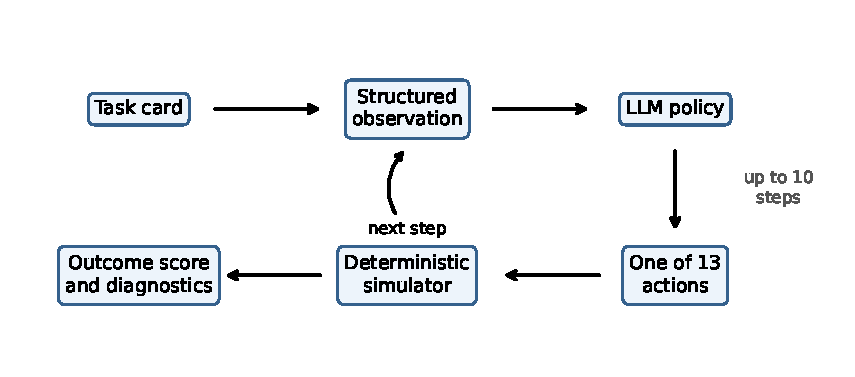
\includegraphics[width=\columnwidth]{figures/benchmark-loop.pdf}
  \Description{A six-stage loop from task card to observation, LLM policy, structured action, deterministic simulator, and outcome score, with repeated simulator steps.}
  \caption{FounderBench interaction loop. Structured actions alter simulator state; only outcomes and documented diagnostics determine task score.}
  \label{fig:loop}
\end{figure}

\subsection{Tasks and families}
The suite contains 50 public tasks, five in each of ten families (Table~\ref{tab:families}): market selection, first revenue, retention, churn recovery, Demo Day traction, pricing, runway preservation, pivot, fundraising, and channel expansion.
FND-001--030 are labeled \texttt{public\_dev} and FND-031--050 \texttt{public\_test}; both sets are released and visible, so the labels support analysis rather than unseen generalization claims.

\begin{table}[t]
\caption{Balanced task-family coverage. Each row contains five tasks.}
\label{tab:families}
\centering\small
\begin{tabular}{ll}
\toprule
Family & Main outcome signals \\
\midrule
Market selection & research, market quality, cash \\
First revenue & customers, revenue, runway \\
Retention & quality, support, retained users \\
Churn recovery & churn, reputation, capacity \\
Demo Day & growth, recurring revenue, cash \\
Pricing & price fit, demand, sustainability \\
Runway & survival, costs, customer base \\
Pivot & diagnosis, market change, recovery \\
Fundraising & traction, credibility, capital \\
Channel expansion & campaigns, partners, scale \\
\bottomrule
\end{tabular}
\end{table}

Tasks are generated from hand-designed synthetic templates with fixed variants and seeds.
They contain no real-company or human-subject records.
This improves control and redistributability at the cost of ecological validity.

\subsection{State, markets, and actions}
Eight synthetic markets differ in demand, competition, willingness to pay, build complexity, support load, and volatility.
Research improves information quality by replacing noisy market signals with exact values.
The 13 actions cover research, offer creation and improvement, campaigns, hiring, support, pricing, interviews, cost cutting, pivots, fundraising, channel partnerships, and no-op.
Exact schemas ship with the artifact.
Because only structured actions execute, a model cannot score by claiming it researched customers or improved a product; it must select the action and pay its simulated cost.

Weekly demand settlement is deterministic given the seeded RNG.
For an offer with awareness $a$, quality $q$, price $p$, and market demand $d$, competition $c$, willingness to pay $w$, and support load $\ell$, acquisition intensity is
\begin{multline}
\lambda_{\mathrm{new}}=\max\!\bigl(0,\,(d\,a\,q\,\mathrm{price\_fit}(p,w)\,r \\
\quad - 0.18c)\,5.5\bigr),
\end{multline}
where $r$ is reputation and $\mathrm{price\_fit}=\max(0.08,1.25-p/\max(1,w))$.
Churn intensity uses
\begin{equation}
\rho=\max\!\bigl(0.01,\,0.08\ell+(0.65-q)\,0.05-0.025r\bigr).
\end{equation}
New and churned customers are drawn from seeded Poisson draws with those rates; cash updates from revenue $p\cdot\mathrm{customers}$ minus support costs and action budgets.
Full action-effect rules are in the appendix and released source.

\subsection{Scoring functions}
Each family implements its own $f_i$.
As concrete examples, market selection uses
\begin{multline}
f=25\min(1,R/3)+55\cdot\mathbf{1}[\mathrm{good\_market}]\\
\quad +20\min(1,\mathrm{cash}/8500),
\end{multline}
where $R$ is the number of researched markets, and first revenue uses
\begin{multline}
f=45\min(1,C/C^\star)+25\min(1,v/v^\star)\\
\quad +20\min(1,\mathrm{cash}/K^\star)+10\min(1,r/0.65),
\end{multline}
with $C$ customers, $v$ peak weekly revenue, and family-specific targets $(C^\star,v^\star,K^\star)$.
Complete component weights for all ten families are in the released rubric and appendix.

\subsection{Design properties}
\label{sec:design-properties}
The desiderata in Section~\ref{sec:desiderata} place FounderBench as a domain-specialized, deterministic-outcome suite within sequential-decision benchmarking~\cite{creus2026agentick}: delayed business consequences matter, but episodes are short, actions are structured, and scores are family-specific rather than oracle-normalized across heterogeneous Gym paradigms.
A natural alternative is \emph{hybrid} verification: keep executable state checks for hard constraints, then grade softer criteria with locked rubrics~\cite{hong2026rulers} or limited expert review.
We prioritize full determinism for v0.3 so every published score is re-executable from the artifact; the cost is reduced ecological validity under market shocks and adversarial conditions that a stochastic or human-in-the-loop layer would capture.

\section{Evaluation Protocol}
\subsection{Metrics}
For task $i$ with final state $x_i$,
\begin{equation}
s_i = \min(100,\max(0,f_i(x_i))).
\end{equation}
The primary aggregate is the unweighted mean $\bar{s}=\frac{1}{50}\sum_{i=1}^{50}s_i$.
A task is solved when $s_i\geq 70$.
We chose 70 as a fixed operating threshold---roughly ``clearly successful'' on the family rubrics---not as an optimized cutpoint: it sits between the generic-heuristic mean (61.01) and the task-aware ceiling (80.90), yields nontrivial but non-saturated solve rates, and keeps solved count complementary rather than redundant with the mean.
We do not ablate alternative thresholds (e.g., 60 or 80) in this paper; average score remains primary because it preserves distances below and above any fixed cut.
We also report median and interquartile range across the 50 task scores to dampen outlier influence.
The table column ``Pub.\ test'' summarizes FND-031--050 only.
Both \texttt{public\_dev} and \texttt{public\_test} are released and visible; the split is for reporting, not a hidden generalization test.
Raw cash and revenue remain diagnostics because tasks differ in initial conditions and objectives.

\subsection{Models and execution}
Hosted APIs use provider-specific adapters under one prompt protocol.
Each task starts from its published seed and state.
Audit mode records traces; a submission validator checks all 50 IDs, score bounds, split summaries, diagnostics, and policy identity before a row enters the paper registry.
Evidence files are frozen by SHA-256.

We evaluate Claude Sonnet 4.5 and 5, DeepSeek Chat and V4 Reasoner, Gemini 2.5 Flash and 3.5 Flash, GLM 4.5 Air, Grok 4.3 and 4.5, GPT-5.6 Sol, and Kimi K3.
Labels record the API identifiers used during collection; they do not imply identical inference settings across providers.
All hosted results are one run per configuration.
We report nonparametric bootstrap intervals over tasks as \emph{task-mix sensitivity}, not sampling variance, and do not use those intervals for significance claims among closely ranked hosted models.

\subsection{Calibration and diagnostics}
\label{sec:calibration}
Four deterministic policies calibrate the suite: random, conservative, generic heuristic, and task-aware heuristic.
They are reference points, not model competitors.
Random samples legal actions; conservative prefers research and support with low spend; the generic heuristic researches markets, builds one offer, then improves quality/awareness/support without using the task family ID.
The task-aware policy additionally branches on family identity (derived from the task ID), e.g., research-then-build for market selection, quality/support focus for retention, hire-then-support for churn shock, price-to-willingness for pricing, cut-cost for runway, pivot when stalled, raise-funding after traction for fundraising, and channel partnership for expansion.
Hosted prompts receive the task card and observation, not an explicit family label; the heuristic's family branch is therefore a privileged prior that ordinary API policies do not share unless the card text leaks family cues.
It approximates a compact family-conditioned strategy and should be read as a calibration ceiling, not as skilled human performance---and not as an unbiased estimate of how large the model gap ``should'' be.
On a frozen private remix of the same families (deterministic calibration only; no hosted private leaderboard), the task-aware mean falls below the generic heuristic (54.81 vs.\ 57.49), consistent with public-suite overfitting risk for that privileged policy.
Released action-space ablations further show that removing quality/support/capacity actions drops the task-aware mean by about 19 points on the public suite, so the ladder depends on the full schema rather than a single silver-bullet action.
The runner records invalid actions, over-budget decisions, provider/parser errors (with categories such as invalid JSON and rate limits), latency, action counts, and token usage when available.
Provider errors trigger documented fallbacks and remain in official scores; we report both raw error decisions and affected-task rates so readers can see interface load without treating official scores as pure strategy.

\section{Results and Analysis}
\begin{table}[t]
\caption{Deterministic calibration policies on the complete suite. The task-aware policy conditions on family identity; see Sec.~\ref{sec:calibration}.}
\label{tab:baselines}
\centering\small
\begin{tabular}{lrr}
\toprule
Policy & Score & Solved \\
\midrule
task\_heuristic & 80.90 & 37/50 \\
heuristic & 61.01 & 19/50 \\
conservative & 54.04 & 13/50 \\
random & 33.30 & 4/50 \\
\bottomrule
\end{tabular}
\end{table}


\subsection{Overall performance}
Calibration policies form a clear capability ladder (Table~\ref{tab:baselines}).
Random scores 33.30 and solves 4/50; the conservative and generic heuristics reach 54.04 and 61.01; the task-aware policy reaches 80.90 and solves 37/50.
The suite is therefore neither trivial nor saturated: structured decision quality and family awareness matter.

\begin{table}[t]
\caption{Validated hosted-model results. Each row is one run over the same 50 public tasks. Median/IQR are across tasks. ``Pub.\ test'' is the FND-031--050 reporting split (also public/visible, not a hidden holdout). Err/aff counts provider-parser error decisions and the number of tasks with at least one such decision.}
\label{tab:models}
\centering\scriptsize
\begin{tabular}{lrrrrrr}
\toprule
Model & Mean & Med. & IQR & Solved & Pub.\ test & Err/aff \\
\midrule
Gemini 3.5 Flash & 67.69 & 80.2 & 27.3 & 32/50 & 59.64 & 59/25 \\
Grok 4.5 & 66.53 & 79.4 & 49.7 & 33/50 & 56.57 & 0/0 \\
GPT-5.6 Sol & 66.39 & 81.6 & 44.8 & 32/50 & 58.42 & 0/0 \\
Kimi K3 & 65.63 & 76.7 & 45.7 & 28/50 & 58.90 & 70/11 \\
Claude Sonnet 5 & 63.90 & 68.5 & 37.1 & 25/50 & 68.61 & 0/0 \\
DeepSeek V4 Reasoner & 62.43 & 75.8 & 55.1 & 27/50 & 58.02 & 3/3 \\
Claude Sonnet 4.5 & 61.09 & 68.0 & 50.4 & 24/50 & 59.58 & 0/0 \\
DeepSeek Chat & 56.59 & 65.5 & 61.6 & 23/50 & 59.70 & 0/0 \\
GLM 4.5 Air & 54.78 & 66.1 & 57.6 & 23/50 & 56.20 & 0/0 \\
Gemini 2.5 Flash & 52.69 & 45.3 & 38.4 & 13/50 & 50.75 & 340/44 \\
Grok 4.3 & 52.59 & 48.5 & 47.7 & 16/50 & 59.43 & 3/3 \\
\bottomrule
\end{tabular}
\end{table}


No hosted single run matches the task-aware ceiling (Table~\ref{tab:models}, Figure~\ref{fig:leaderboard}).
The top of the hosted table is a tight cluster rather than a decisive ranking: Gemini 3.5 Flash has the highest single-run average at 67.69 (task-mix 95\% interval $[59.20,75.25]$), followed closely by Grok 4.5 at 66.53 ($[57.81,74.62]$) and GPT-5.6 Sol at 66.39 ($[57.46,74.89]$).
These intervals overlap almost completely, so the 1.3-point Gemini--GPT gap is not a significant separation under task-mix resampling.
Grok 4.5 solves the most tasks (33/50), while Gemini and GPT both solve 32/50.
Several models clear half the suite, so the environment is tractable, but the best hosted average remains more than 13 points below task-aware calibration.

\begin{figure}[t]
  \centering
  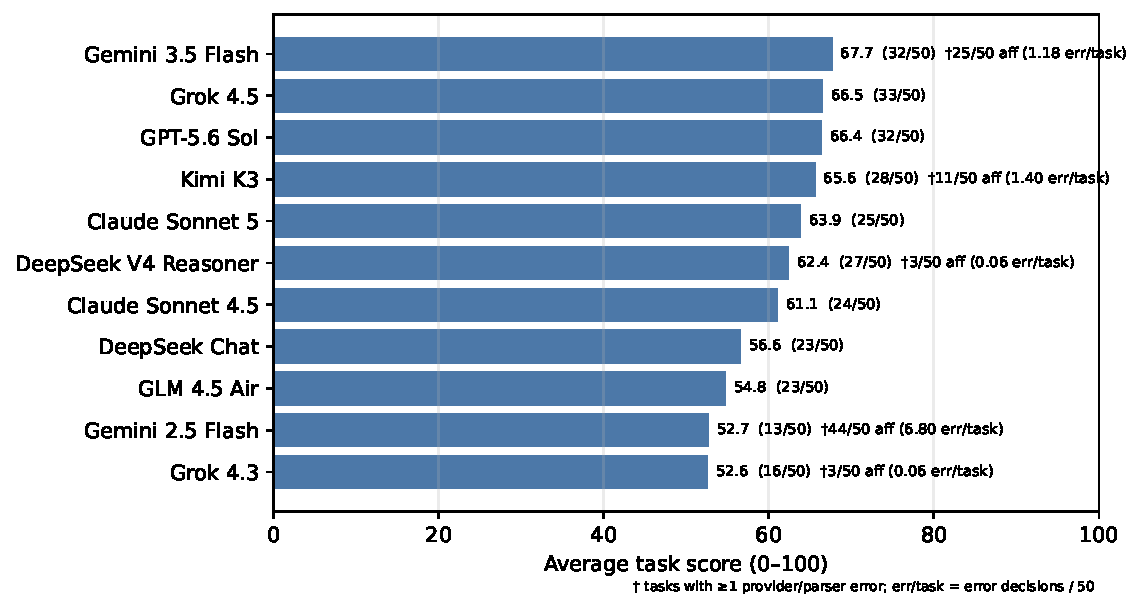
\includegraphics[width=\columnwidth]{figures/model-leaderboard.pdf}
  \Description{Horizontal bars compare average task scores for validated hosted models, annotated with solved counts and provider-error markers.}
  \caption{Validated hosted single-run leaderboard. Daggers report affected-task counts and error decisions per task; raw counts alone are not severity.}
  \label{fig:leaderboard}
\end{figure}

\subsection{Solved count versus average score}
Solved count and average score answer different questions.
Once a task crosses 70, solved count discards further gains; average score still rewards raising 70 to 90 and penalizes severe failures.
Rank reversals follow: Gemini 3.5 Flash outscores Grok 4.5 on average but solves one fewer task; similar reversals appear for Claude Sonnet 5 versus DeepSeek V4 Reasoner and Gemini 2.5 Flash versus Grok 4.3.
We therefore treat average score as primary and solved count as complementary.

\subsection{Close top models and cross-benchmark rankings}
FounderBench rankings need not match public LLM leaderboards that emphasize coding, chat, or general reasoning.
Pairwise, Gemini 3.5 Flash and GPT-5.6 Sol win 21 and 19 tasks respectively (10 ties); their advantage is concentrated in different families (e.g., Gemini on Demo Day and pivot, GPT on channel, churn recovery, and runway).
Split summaries also disagree with a single ``best model'' story: Claude Sonnet 5 has the strongest \texttt{public\_test} average (68.61) despite a mid-table overall mean.
Moreover, Gemini's top average coexists with 59 provider/parser error decisions (invalid JSON and rate limits), so the row is not a clean strategic win.
Together with the overlapping task-mix intervals, these facts advise reading the top hosted rows as a near-tie on this suite---not as evidence that Gemini Flash dominates GPT-class models in general.

Cross-benchmark agreement with long-horizon CEO sims should likewise not be assumed.
CEO-Bench~\cite{chen2026ceobench} and YC-Bench~\cite{he2026ycbench} stress sustained coherence over hundreds of days/turns with ending cash as the scalar, whereas FounderBench measures family-conditioned operating quality over short episodes.
A model that ranks well on FounderBench may still fail a 500-day cash game, and vice versa; we therefore treat Section~5 as suite-local evidence rather than a substitute for those long-game evaluations.
Benhenda's forecasting YC Bench~\cite{benhenda2026ycbenchforecast} further motivates reporting multiple aggregates (mean, median/IQR, solved count, family profiles): different ``outcome'' notions answer different questions about startups.

\subsection{Family-level behavior and failure taxonomy}
Figure~\ref{fig:heatmap} shows that similar overall scores can hide different operating profiles.
Some models do relatively well on runway or retention yet struggle on pivots and fundraising, where early actions create later prerequisites.
The task-aware policy exceeds the best hosted family mean on eight of ten families; hosted models lead only on retention improvement and churn shock recovery.
Each cell averages only five synthetic visible tasks and reports within-cell standard deviation; small differences should not be overread as stable capability gaps.

\begin{figure*}[t]
  \centering
  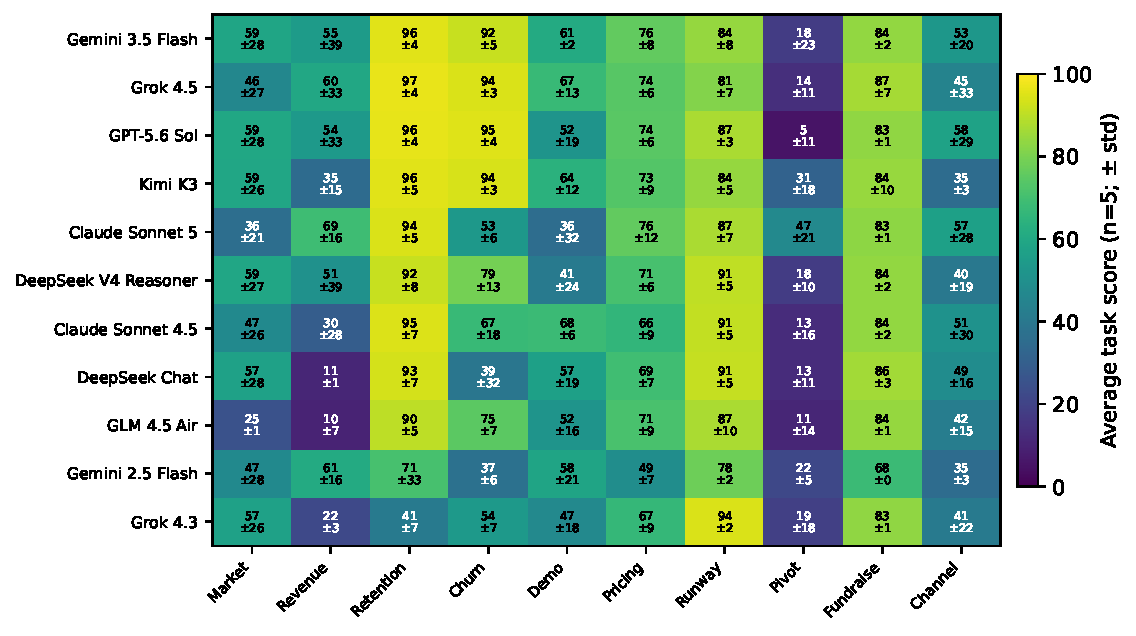
\includegraphics[width=0.92\textwidth]{figures/family-heatmap.pdf}
  \Description{A heatmap shows average scores for each hosted model across ten startup operating task families, with per-cell standard deviation.}
  \caption{Average score by hosted model and task family ($n{=}5$ tasks per cell; cell text shows mean$\pm$std). Diagnostic only.}
  \label{fig:heatmap}
\end{figure*}

Observed failures concentrate in four recurring buckets (descriptive, not mutually exclusive):
\begin{itemize}
  \item \textbf{Prerequisite gaps.} Pivot and Demo Day show the largest task-aware--hosted gaps (about 18 and 21 points at the best hosted family mean), consistent with missing early research/improve sequences that unlock later recovery.
  \item \textbf{Budget and runway mistakes.} Runway and fundraising require timed \texttt{cut\_cost}/\texttt{raise\_funding}; models often campaign or hire before stabilizing cash.
  \item \textbf{Family misfit.} Retention/churn are where hosted models can match or exceed the task-aware prior, suggesting the public ladder is not uniformly hard and that ``average score'' alone hides specialization.
  \item \textbf{Interface load.} Provider/parser failures remain in official scores: Gemini 2.5 Flash records 340 error decisions on 44/50 tasks; Kimi K3 records 70 on 11 tasks; Gemini 3.5 Flash's top average coexists with 59 errors (see the appendix provider-error table).
\end{itemize}
These buckets motivate reporting family profiles and error rates alongside the mean: a high average can still hide prerequisite failures or dense API fragility.

\subsection{Provider-error sensitivity}
Official scores retain provider and parser failures because interface reliability is part of end-to-end execution.
We also stratify each run into tasks with and without recorded errors and normalize by reporting error decisions per task and the fraction of affected tasks (appendix provider-error table).
This stratification is descriptive, not counterfactual: the subsets contain different tasks, so mean differences do not estimate an error-free score, and we do not yet provide an interface-only retry ablation.
Gemini 3.5 Flash's affected-task mean is higher than its unaffected mean, which is exactly why the split cannot be treated as a causal penalty.

\section{Reproducibility and Responsible Use}
The release includes Python source, task definitions, simulator and scoring code, adapters, a resumable runner, raw task-level JSON, submission reports, generated tables and figures, a benchmark card, datasheet, task cards, scoring rubric, prompt protocol, environment report, and checksums.
Documentation follows datasheet and holistic-evaluation practice~\cite{gebru2021datasheets,liang2023holistic}.
Deterministic baselines run without commercial credentials; hosted reproduction requires provider keys and may drift with API updates.

For dataset-and-benchmark review, we emphasize:
\emph{accessibility} of a self-contained package with key-free baselines;
\emph{documentation} of actions, rubrics, and schemas;
\emph{impact} as a shared test bed for resource allocation and recovery rather than business-plan prose;
\emph{bounded representativeness} of balanced synthetic families;
\emph{reproducibility} via fixed seeds, raw outcomes, hashes, and generators; and
\emph{responsible use} through synthetic data plus explicit bans on investment or deployment claims.

Accessibility still depends on final public repository and license metadata.
Any post-result task or rubric change must create a new version rather than silently alter the reported suite.

The release also freezes a 20-task private holdout (two tasks per family), with public fingerprint commitments and an evaluator-held secret.
Private task definitions are not published; all hosted results in this paper are on the visible public suite, so there is no official hidden leaderboard of model scores.

\section{Limitations}
\textbf{Synthetic validity.}
Hand-designed, largely deterministic transitions approximate only a subset of startup dynamics and omit market shocks, adversarial feedback, and many stochastic couplings that would miscalibrate difficulty relative to real operations.
Passing does not imply real-market judgment; seeded noise variants and broader templates would improve ecological coverage.

\textbf{Visible public suite and contamination.}
All 50 public task definitions are released; \texttt{public\_test} is a reporting split, not a hidden exam.
A frozen private task list exists for contamination-resistant evaluation, but this paper does not report hosted scores on it, so there is no official hidden leaderboard.
Without repeated hosted runs or private hosted scores, sampling variance and contamination risk remain only partially quantified.

\textbf{Single hosted runs and missing protocol ablations.}
Task-mix intervals do not capture sampling variance, provider drift, or repeated-run reliability, so close leaderboard gaps are fragile.
We also lack systematic ablations of prompt protocols, action-schema variants for hosted models, alternative solve thresholds, and sensitivity sweeps over observation-noise intensity or cost coefficients.

\textbf{Provider dependence versus strategy.}
Availability, rate limits, aliases, and formatting affect end-to-end scores; because provider/parser errors remain in official means, strategic competence is partially conflated with API/adaptor robustness.
Diagnostics expose load (affected tasks, err/task) but cannot fully disentangle infrastructure and strategy without a standardized retry or interface-only ablation.

\textbf{Calibration priors.}
The task-aware heuristic encodes family-specific priors and can overfit the visible suite; the hosted-to-task-aware gap should not be over-interpreted as pure strategic deficit.
There is no human-founder calibration, no official hidden leaderboard, and no comparison of scores against founder or domain-expert decisions.
The 80.90 task-aware score is therefore a synthetic ceiling, not a human reference.

\textbf{Representativeness.}
Ten balanced families omit legal, accounting, ethics, security, and many domain-specific decisions.
Hiring is a single coarse action rather than the managerial lifecycle studied by AgentHire-Bench~\cite{agenthire2026}; reputation shocks are milder than BrandEval-style crisis communication~\cite{brandeval2026}.

\section{Conclusion}
FounderBench asks whether agents can turn noisy observations into consequential startup-like actions under bounded resources.
Its central design choice is to score deterministic simulated outcomes rather than persuasive prose.
Eleven hosted configurations show substantial capability but remain below a task-aware calibration policy, with heterogeneous family behavior and solved-versus-average rank reversals.
The release ties every reported number to executable evidence.
FounderBench should be read as a controlled synthetic sequential-decision test---not a predictor of company success.
Priority upgrades are repeated hosted runs, private hosted evaluation, interface-retry and environment-sensitivity ablations, and expert/founder calibration.

\bibliographystyle{ACM-Reference-Format}
\bibliography{../../outputs/founderbench-references}

\end{document}
